\chapter{Background}

This chapter provides background knowledge regarding software architecture and architectural security constraints. The ArchUnit library is introduced and related to tools and approaches used in previous research.

\section{Software architecture}
The intention of this study is not to contribute to the definition of software architecture, though, our work relies on a shared understanding of what constitutes as the architecture of a system. This section presents the concept of software architecture and the definitions considered in our study.   

During the 1970s,  the idea of organizing software into distinguishable structures was initially introduced. Djikstra \cite{dijkstra_structure_1968} organized the system into a hierarchy of layers, each being dependent upon the interface of the layer below. Parnas discussed the criteria used to modularize systems \cite{broy_criteria_1972}, i.e. responsibility assignment, which allowed for independent development. Further, he introduced the concept of program families \cite{parnas_design_1976} where a set of systems share much of their functionality, allowing for a common design. The work on product families was later extended to describe the process of designing systems that support extensions by using abstracted components \cite{parnas_designing_1979}. 

However, the term \textit{software architecture} was formally introduced by Perry and Wolf in \cite{perry_foundations_1992}, where they defined software architecture as:

\[ Software \;  Architecture = \{elements,form,rationale\} \]

In words, software architecture is defined as a set of architectural elements that persist in a particular form. Form relates to the properties of each element and the relationship between elements. To make an architecture explicit, Perry and Wolf \cite{perry_foundations_1992} suggest the usage of views to represent different aspects of the architecture. 

Related to that of a specific architecture, Perry and Wolf \cite{perry_foundations_1992} define an architectural style as a generalization of various similar architectures. Garlan and Shaw \cite{ambriola_introduction_1993} extended the knowledge by providing a list of architectural styles that were commonly used in the design of software systems, these include \textit{pipes and filters}, and \textit{layered systems}. Perhaps more importantly, Garlan and Shaw \cite{ambriola_introduction_1993} describe the rationale of using a specific style and the trade-offs between styles.

Today, there are mainly two definitions of software architecture:

\begin{itemize}
    \item \textbf{Bass et Al \cite{bass_software_2013}}: \say{The software architecture of a program or computing system is the structure or structures of the system, which comprise software elements, the externally visible properties of those elements, and the relationships among them.}
    \item \textbf{Jansen and Bosch \cite{jansen_software_2005}}: \say{The composition of a set of architectural design decisions} where a design decision represents \say{A description of the set of architectural additions, subtractions and modifications to the software architecture, the rationale, and the design rules, design constraints and additional requirements that (partially) realize one or more requirements on a given architecture.}
\end{itemize}

While both definitions acknowledge that a system should always meet the functional requirements and that the process of creating the architecture is a balance between quality attributes, it is the former definitions that lend itself naturally to structural analysis.

Finally, in many references to architecture, the term design is often used ambiguously. To remedy this, Eden and Kazman \cite{eden_architecture_2003} formalized the hypothesis of an intension and locality criteria. A specification is said to be intensional if there are infinitely many ways of realization, all others are extensional. Further, a specification is said to be local if it only affects a small part of a program. Architectural specifications are both intensional and non-local, whereas design level specifications are intensional and local.

\section{Architectural security constraints}

The purpose of software and architectural security is to ensure that no harm occurs to the systems assets in the presence of malicious actors \cite{mcgraw_software_2004}. Assets are identified by the needs of the systems stakeholders and may be tangible (e.g, cash) or intangible (e.g, information) \cite{haley_security_2008}. At the core of software security are the following four concerns, often refereed to as CIAA:

\begin{itemize}
    \item \textbf{Confidentiality}, \say{Preserving authorized restrictions on information access and disclosure.} \cite{ross_systems_2018}
    \item \textbf{Integrity}, \say{Guarding against improper information modification or destruction.} \cite{ross_systems_2018}
    \item \textbf{Availability}, \say{Ensuring timely and reliable access to and use of information.} \cite{ross_systems_2018}
    \item \textbf{Accountability}, \say{Ensuring that it is possible to trace security relevant actions (i.e., subject-object interactions) to the entity on whose behalf the action is being taken} \cite{ross_systems_2018}
\end{itemize}

These concerns relate to a system's security goals as a violation of a concern to one of the assets describes a possible threat \cite{haley_security_2008}. Security requirements later operationalize the security goals and constrain the architecture of a system. As security is often considered a quality attribute, the satisfaction of a security requirement becomes a risk management issue.  Highly valuable assets should warrant a higher degree of protection and consequently, require stronger constraints on the architecture \cite{broy_software_2007}.

While the term architectural constraint means refers specifications that impact the structures of a system, and the relationships between them, several concepts and techniques have come to form a generalizable knowledge of solutions, at different levels of abstraction, that serve as constraints to satisfy the requirements. The concepts outlined below have definitions that vary across authors; thus, our goal is not to provide conclusive definitions but rather an overview. 

\textbf{Security principles}, such as those proposed by OWASP\footnote{\url{https://blog.threatpress.com/security-design-principles-owasp/}}, are defined at a level of high abstraction that allows them to be used on almost any component in a system. Examples of such principles include \textit{The principle of least privilege}, stating that any user should have the least amount of privileges needed to perform an action. While the abstraction of principles enables them to apply to most components of a system, it also means that an architect has to assess, instead of precisely knowing, whether the constructed architecture conforms to the principle. 

\textbf{Architectural tactics}, introduced by Bass et al in \cite{bass_software_2003}, refers to \say{a design decision that influences the achievement of a quality attribute respone}. In particular, security tactics aim to control the security response of a system, i.e. ensuring that the security goals always hold true. The original list of security tactics has later been refined \cite{ryoo_revising_2012,fernandez_revisiting_2015} and includes techniques for detecting, resisting, reacting to and recovering from attacks, as seen in Figure~\ref{fig:security_tactics}. Much like principles, tactics lack a common realization causing the architect to subjectively asses whether the tactic is implemented.

\begin{figure}
    \centering
    \captionsetup{justification=centering}
    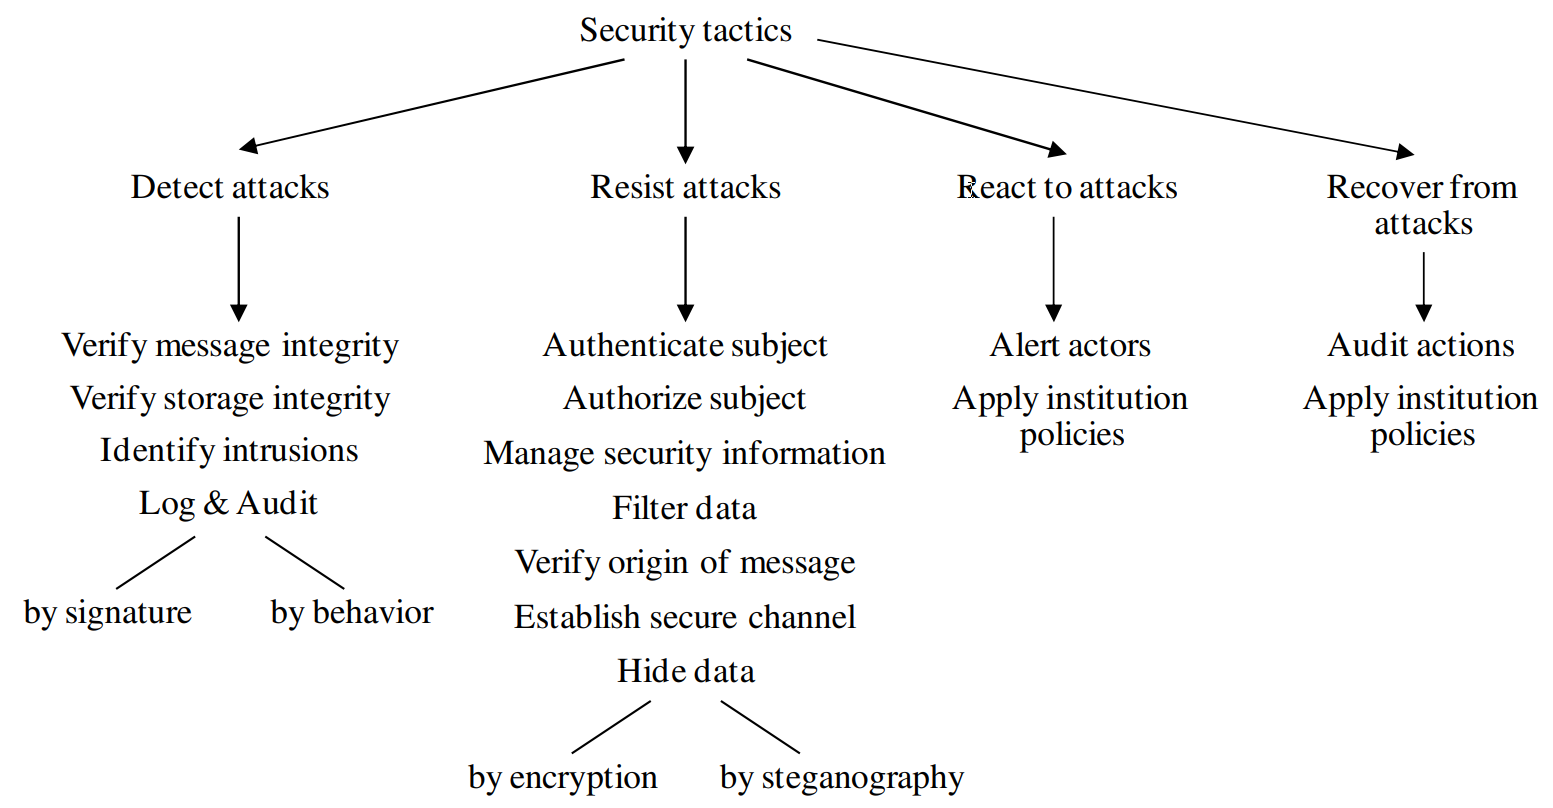
\includegraphics[width=\textwidth]{figure/securityTactics.png}
    \caption{A hierarchical tree of security tactics, adapted from \cite{fernandez_revisiting_2015}.}
    \label{fig:security_tactics}
\end{figure}

\textbf{Security patterns} are at a lower level of abstraction as they represent \say{encapsulated solutions to recurrent system problems} \cite{fernandez-buglioni_security_2013}. By composing a set of tactics in a generalizable solution to a known problem, patterns help to bridge the gap between the developers and the architectural experts \cite{rosado_study_2006}. The extensive knowledge of security patterns and their implementation also allows for comparisons in terms of their impact on other quality attributes, such as maintainability and performance \cite{scandariato_architecting_2009}. 

\textbf{Security rules}, while not as established in the literature, has come to serve as a less solution-oriented version of patterns. Rules often define dependencies, such as \say{Layer X must not access layer Y}, but may also define behavioral aspects. Much of the commonly used rules are tacit knowledge, meaning that there are few explicit mentionings. 

\section{ArchUnit}\label{archunit-back-section}
ArchUnit is a library that leverages static analysis to validate architectural constraints. Static analysis refers to the analysis of code, either in the shape of source code or compiled bytecode, without executing the code itself \cite[p. 21]{chess_secure_2007}. In the case of ArchUnit, the analysis is performed on compiled Java bytecode.

Using ArchUnit, a target system can be analyzed and composed into a Java code structure \cite{gafert_archunit_2020}. This structure contains a number of classes, outlined in Figure~\ref{fig:archunit}, which describe the code of the analyzed system. Some key observations regarding this structure:

\begin{figure}
    \centering
    \captionsetup{justification=centering}
    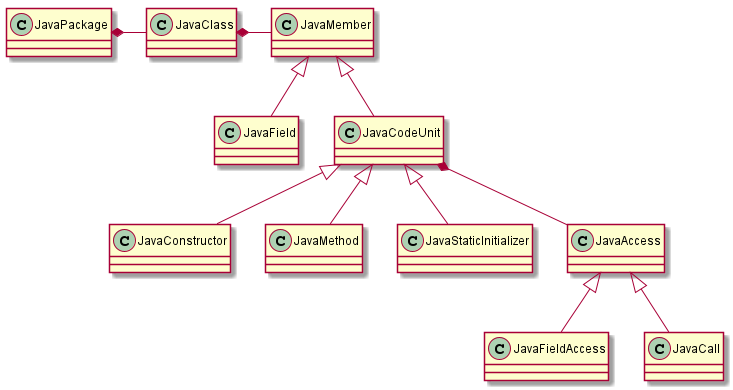
\includegraphics[width=\textwidth]{figure/ArchUnit.png}
    \caption{The architectural constructs present in the domain of ArchUnit, adapted from \cite{gafert_archunit_2020}.}
    \label{fig:archunit}
\end{figure}

\begin{itemize}
    \item Methods, constructors and static initializers, i.e. anything that contains code statements, are collectively referred to as \textbf{code units}.
    \item Fields and code units, i.e. constructs that are owned by a class, are referred to as \textbf{members} of that class.
    \item Field accesses, method calls and constructor calls are collectively known as \textbf{accesses}. An access has a source, i.e. the code unit from which the access originates, and a target, i.e. the member that is being accessed.
\end{itemize}

The validation of a constraint is performed by evaluating one or multiple conditions against select properties of this code structure. ArchUnit exposes a sentence-like API that allows these constraints to be expressed as sentences of the form \say{The \textbf{constructs} that match \textbf{predicate} should fulfill \textbf{condition}.} 

An example of a constraint can be seen in Listing~\ref{lst:architectural_rule}. This constraint assumes that there are two layers \textit{view} and \textit{controller}, in the form of packages, and dictates that the view layer should only be accessed by the controller layer. In this example, the constructs are classes (line 1), the predicate selects classes declared in a package with the suffix \textit{view} (line 2), and the conditition applied to these classes is that they should only be accessed by code units declared in a package with the suffix \textit{controller} (line 3).

\begin{center}
\begin{minipage}{0.90\linewidth}
\begin{lstlisting}[caption={Example of an architectural rule in ArchUnit.}, captionpos=b, label=lst:architectural_rule, numbers=left]
ArchRule rule = classes()
    .that().resideInAPackage("..view")
    .should().onlyBeAccessed().byAnyPackage("..controller");
\end{lstlisting}
\end{minipage}
\end{center}

In general, constructs refer to either classes or members. It is also possible to select a specific type of member, such as fields or constructors. The predicate is used to filter constructs based on their attributes, such as selecting classes that are defined in a specific package as seen in the example above. Finally, the condition is applied to all the selected constructs. Constructs that fail to fulfill the condition are reported as violating the constraint.


% \cite{pistoia_survey_2007}

% constraints can be enforced both statically and dynamically, as covered in related work
% ArchUnit employs static analysis; explain briefly what it means
% This, combined with constraints that can be validated with unit testing infrastructure, enables the tool to be used as part of a continuous integration pipeline
% These constraints are expressed in Java code and can be validated using conventional unit testing frameworks. 


\section{Related work}
This section presents existing approaches to architectural conformance monitoring and notations for expressing security concerns, and how they relate to this work.

\subsection{Architectural conformance monitoring}

In one approach to architectural conformance monitoring called ArchJava, presented by Aldrich et al. \cite{aldrich_archjava_2002}, the Java language is extended with syntax for describing architectural elements such as components and connectors. Constraints on these architectural elements are validated at compile-time, allowing violations to be caught at an early stage of development.

Abi-Antoun and Barnes \cite{abi-antoun_analyzing_2010} present a two-tiered approach to architectural conformance monitoring called SECORIA. Their approach utilizes code annotations and static analysis to extract an architectural representation of a system. This representation is then compared to a target architecture, which is modeled separately in an Architecture Description Language (ADL), in order to detect discrepancies between the intended architecture and the actual implementation.

De Silva \cite{de_silva_towards_2014} presents PANDArch, another two-tiered approach, in which the intended architecture is modeled using an ADL and checked for conformance with the actual implementation. As opposed to SECORIA, PANDArch utilizes dynamic analysis to extract the implemented architecture during executions of the system. 

The approach used by ArchUnit allows architectural constraints to be expressed directly in the source code, replacing the need for a separate model of the intended architecture. In addition, these constraints can be validated using existing unit test runners, enabling the tool to be used as part of a continuous integration pipeline.

%Comparison of static approaches
%\cite{knodel_comparison_2007}

%\cite{luckham_event-based_1995}
%\cite{de_silva_controlling_2012}



\subsection{Design annotations and security notations}

Sabo and Porubän \cite{sabo_preserving_2009} use Java annotations to preserve the correct form of design patterns during implementation. While the approach does not focus on security, the study showcases how constraints can be applied directly to the source code. Additionally, Sabo and Porubän argue that storing constraints at the location of its implementation increases developer awareness. 

Similarly, Sulir et al. \cite{sulir_recording_2016} record the developer's intentions (including security concerns) using source code annotations. They showed through two controlled experiments that annotations helped improve program comprehension and the correctness of the implementation.

Both SecureUML by Lodderstedt el al. \cite{goos_secureuml_2002} and UMLsec by Jürjens \cite{goos_umlsec_2002} propose extensions to UML to incorporate security-relevant information to allow for formal reasoning and evaluation. While SecureUML focuses solely on access control, specifically role-based access control, UMLsec provides more general constructs.

While SecureUML and UMLsec define concepts at a relatively low level of abstraction to allow for the generation of access control infrastructure for the former, and formal verification for the latter, Sion et al. \cite{sion_masc_2015} propose another set of extensions aimed at concerns on the architectural level. The extensions are based on two sets of security design concepts: (1) \say{well-known and often-used security concepts or techniques} and (2) \say{security goals and objectives}. As a consequence of the focus on architectural level concerns, much of their extension to UML are graphical elements rather than stereotypes and tagged values, as in the previous examples. 

A systematic review of the field by van den Berghe et al. \cite{vandenberghe_design_2017} revealed that of the many proposed notations for security, few had any existing tool support outside of a vaguely mentioned prototype. Additionally, the coverage across security concerns was not equal. Most notations covered aspects of access-control but lacked support for most of the CIAA concerns. 

Our approach tries to extend the field of security notation by applying them to architectural conformance testing. We utilize annotations, in the shared belief of \cite{sabo_preserving_2009} that constraints should be applied closest to their implementation. While the use of formal models allows for rigorous proofs, we believe a more lightweight model can be a complement in settings where formality becomes too large of an overhead, such as in agile environments. 